%\documentclass{sigplanconf}
\documentclass[preprint,nocopyrightspace]{sigplanconf}

\usepackage{amsmath}
\usepackage{amssymb}
\usepackage{textcomp}
\usepackage[usenames]{color}
\usepackage{graphicx}
\usepackage{url}
\usepackage{rotating}
\usepackage{multirow}
\usepackage{booktabs}
\usepackage{listings}
\usepackage{array}
\usepackage[T1]{fontenc}
\usepackage{luximono}

\newenvironment{packed_enum}{
\begin{enumerate}
  \setlength{\topsep}{0pt}
  \setlength{\itemsep}{5pt}
  \setlength{\parskip}{0pt}
  \setlength{\parsep}{0pt}
}{\end{enumerate}}

\newenvironment{packed_itemize}{
\begin{itemize}
  \setlength{\topsep}{0pt}
  \setlength{\itemsep}{5pt}
  \setlength{\parskip}{0pt}
  \setlength{\parsep}{0pt}
}{\end{itemize}}

\newcommand{\todo}[1]{{\color{red} \bf [TODO: #1 ]}}


\lstdefinelanguage{Scala}{
  morestring=[b]",
  morestring=[b]',
  morecomment=[l]{//},
  morecomment=[s]{/*}{*/},
  morekeywords={var,val,def,private,class,object,trait,implicit,if,else,new,do,while,@volatile,try,catch,case,match,throw,return,extends,with,import}
}

\lstset{
  language=Scala,
%  basicstyle=\fontsize{7.5}{9}\selectfont\tt,
  basicstyle=\fontsize{7}{8}\selectfont\tt,
%  basicstyle=\selectfont\tt,
  keywordstyle=\bfseries,
  numbers=left,
  numberstyle=,
  commentstyle=\itshape,
  columns=fixed,
  xleftmargin=0.25in,
  firstnumber=auto,
  escapechar=\#,
  emph={A,B,C,K,V,U,Z}, emphstyle=\bfseries\itshape,
  emph={[2]Unit,Int,Set,Map,TSet,TMap,TVar,Option,Boolean,Txn,Money,Account,OverdraftException,Ref,Source,Sink,Bound,ReadResource}, emphstyle={[2]\itshape}
}

\newcommand{\code}[1]{{\fontsize{8}{9.5}\selectfont \tt #1}}
\newcommand{\codesec}[1]{{\fontsize{10}{12}\selectfont \tt \bfseries #1}}
\newcommand{\codeft}[1]{{\fontsize{6.5}{8}\selectfont \tt #1}}
\newcommand{\type}[1]{{\code{\itshape #1}}}
\newcommand{\typesec}[1]{{\codesec{\itshape #1}}}
\newcommand{\typeparam}[1]{{\code{\bfseries #1}}}
\newcommand{\typeparamsec}[1]{{\codesec{\bfseries #1}}}
\newcommand{\xtype}[2]{{\type{#1}\typeparam{[#2]}}}
\newcommand{\xtypesec}[2]{{\typesec{#1}\typeparamsec{[#2]}}}
\newcommand{\ytype}[2]{{\type{#1}\code{[}\type{#2}\code{]}}}
\newcommand{\xxtype}[3]{{\type{#1}\typeparam{[#2,#3]}}}
%\newcommand{\keyword}[1]{{\code{\bfseries #1}}}
\newcommand{\keyword}[1]{{\code{#1}}}

\hyphenation{CC-STM}
\hyphenation{Deuce-STM}
\hyphenation{Mul-ti-verse}

\begin{document}

\conferenceinfo{Scala Workshop,}{April 15, 2010, Lausanne, Switzerland.}
\CopyrightYear{2010}
\copyrightdata{}

\newcommand{\xtitle}[0]{CCSTM: A Library-Based STM for Scala}
\newcommand{\xterms}[0]{{Algorithms, Languages}}
\newcommand{\xkeywords}[0]{{Transactional memory, Scala}}
%\titlebanner{[WORK IN PROGRESS: Do Not Circulate!]}        % These are ignored unless
\preprintfooter{\xtitle}  % 'preprint' option specified.

\title{\xtitle}

\authorinfo{Nathan G. Bronson \and Hassan Chafi \and Kunle Olukotun}
           {Computer Systems Laboratory\\
            Stanford University}
           {\textit{\{nbronson, hchafi, kunle\}@stanford.edu}}

\pdfinfo{
  /Title    (\xtitle)
  /Author   (Nathan G. Bronson and Hassan Chafi and Kunle Olukotun)
  /Subject  (\xterms)
  /Keywords (\xkeywords)
}

\maketitle

\begin{abstract}

We introduce CCSTM, a library-based software transactional memory (STM)
for Scala, and give an overview of its design and implementation.
Our design philosophy is that CCSTM should be a useful tool for the
parallel programmer, rather than a parallelization mechanism for arbitrary
sequential code, or the sole synchronization primitive in a system.

%This frees us from the semantic tar pits that surround privatization,
%strong isolation, and irrevocable system calls.

CCSTM expresses transactional reads and writes as explicit method calls on
instances of a reference type.  Scala's flexible method names, implicit
parameters, and closures keep the syntax concise, and the reference
instances provide a natural way to express additional STM functionality.
We use a novel hybrid of static and dynamic transaction scoping to
retain composability while avoiding the barrier overheads that would
otherwise result from an implementation as an unprivileged library.
Experiments show that CCSTM's performance and scalability are
on par with bytecode rewriting STMs.


%Transactional accesses in CCSTM are performed via explicit method calls
%on instances that implement a trait \type{Ref}.  These transactional
%references may be long-lived, or may be transient accessors to bulk
%transactional data such as an array.  Scala's operator overloading keeps
%the syntactic overhead low for basic reads and writes.  The \type{Ref}
%trait serves as a first-class representation of a transactionally-managed
%memory location, providing a natural way to express additional STM
%functionality such as modular blocking, non-transactional compare-and-swap,
%manually-validated reads, and deferrable transformation using pure
%functions.
%
%In an additional departure from typical STM designs, CCSTM uses a
%hybrid of static and dynamic transaction scoping.  \type{Ref}'s methods
%are bound to current transaction via a \keyword{implicit} parameter.
%When an atomic block is entered, however, nesting is resolved dynamically.
%This hybrid approach avoids the overheads of a dynamic lookup for most
%STM operations without requiring the transaction to be statically threaded
%throughout the user's code.

\end{abstract}

\category{D.1.3}{Programming Techniques}{Concurrent Programming -- Parallel programming}
\category{D.4.1}{Operating Systems}{Process Management -- Concurrency; Synchronization; Threads}

\terms
\xterms

\keywords
\xkeywords

\section{Introduction}
\label{sec:intro}
The proliferation of multi-core processors means that more programmers are
being thrust into the difficult world of shared memory multi-threading.
\todo{a couple sentences more of boilerplate motivation}

Software transactional memory (STM) provides a compelling alternative to
locks for managing access to shared mutable state.  STM's declarative
atomic blocks are free from deadlock, are composable, and do not
require elaborate fine-grained decomposition to yield scalability.
These benefits stem from an optimistic execution strategy that includes
rollback and retry, allowing the runtime to attempt concurrent execution
based only on a likelihood of success.  STMs bridge the gap between their
simple programming model and their speculative execution by isolating
uncommitted transactions from the rest of the system.  Most of the
difficulty in integrating an STM into a language comes from tradeoffs
between the overhead, fidelity, and complexity of this isolation.

In this paper we describe the design of CCSTM, a library-based STM for
Scala.  CCSTM deliberately sidesteps many of the performance and semantic
difficulties common in software implementations of transactional memory
by limiting its focus: CCSTM is a tool for use by parallel programmers
that wish to build algorithms and data structures using optimistic
concurrency control, not an all-encompassing concurrent programming
model or a mechanism for automatic parallelization of arbitrary code.

The most fundamental design choice for CCSTM was the decision to
implement it entirely as a Scala library.  Unlike STMs that instrument
normal loads and stores, transactional accesses in CCSTM are explicit
method calls to a Scala \xkeyword{trait}\footnote{Property accessors
may used to eliminate the syntactic overhead for many situations.}.
We refer to the resulting STM as `reference-based', because all memory
locations managed by the STM are boxed inside transactional references.
Both transactional and non-transactional access to the managed references
goes through methods implemented by instances of this \xtypeA{Ref}.

While a reference-based STM imposes a syntactic burden for simple loads and
stores, it also makes the STM more expressive.  A \xtype{Ref} provides
a first-class object that names a memory location, something that would
otherwise require reflection in Scala.  In addition, the reference provides a
convenient namespace for additional STM functionality, such as semantic
conflict detection or transformation by an associative function.
%As a
%practical benefit, the extra level of indirection provided by \xtype{Ref}
%allows multiple implementations, allowing tradeoffs between the cost of
%validation and the likelihood of rollback.

CCSTM's second departure from the typical STM interface is to bind the
transaction scope statically, rather than dynamically.  Transactional access
methods in \xtype{Ref} take an implicit parameter of type \xtype{Txn}, and
perform their accesses in the context of that transaction.  This decision
was made for pragmatic reasons, because performing a dynamically-scoped
lookup on each transactional access would be prohibitively expensive.

A useful parallel can be made between Haskell's STM [[ref]] and CCSTM.
Haskell's \xtype{TVar} corresponds to instances of type \xtype{Ref}.
\xtype{Txn} is not a monad, but it proliferates through STM-enabled
methods in exactly the same way as the \xtype{STM} monad.

In this paper, we:
\begin{packed_enum}

\item We describe CCSTM, a reference-based STM for Scala.  CCSTM focuses on
helping parallel programmers build optimistically concurrent algorithms
and data structures, while restricting itself to implementation techniques
that do not interfere with components of the system that do not use it
(Section~\ref{fig:?}).

\item We introduce \xcode{unrecordedRead}, a new STM primitive that can be coupled with
transaction life-cycle callbacks to provide semantic conflict detection.  We use
unrecorded reads to add a \xcode{map(f)} method to \xtype{Ref} that performs
conflict detection on the result of applying \xcode{f}, rather than on the
transactional value (Section~\ref{fig:?}).

\item We summarize the discussions that led from the original design goal to
the current syntax.  We point out the parts that work well and the parts that
are burdensome, and hypothesize about ways to address the latter
(Section~\ref{fig:?}).

\item We compare the performance of CCSTM to Multiverse and DeuceSTM, STMs for
the JVM that use bytecode rewriting.  We find that CCSTM's implementation as an
unprivileged library does not impose a performance penalty
(Section~\ref{fig:?}).  \todo{is this true}

\end{packed_enum}



\begin{figure}
\begin{lstlisting}{name=Code}
class Account(initialBalance: Money) {
  private var _balance = initialBalance

  def balance: Money = _balance

  def deposit(amount: Money): Unit = {
    assert(amount >= 0)
    _balance += amount
  }

  def withdraw(amount: Money): Unit = {
    assert(amount >= 0)
    if (_balance < amount)
      throw new OverdraftException
    _balance -= amount
  }
}

object Account {
  def transfer(src: Account, dst: Account,
        amount: Money): Unit = {
    src.withdraw(amount)
    dst.deposit(amount)
  }
}
\end{lstlisting}

\caption{Code that performs an account transfer without
any locking or other concurrency control.}

\label{fig:example:nosync}
\end{figure}


\section{Motivation}
\label{sec:library}

An experimental feature such as software transactional memory should
strive to impose only negligible costs on code that does not use it.
Runtime performance costs are the most obvious, but extra complexity in
the compiler, libraries, and language rules should be minimized.
A pay-as-you-go philosophy facilitates incremental adoption, it allows
multiple implementations to coexist, and it reduces the penalty for
failure.

One popular and reasonable interface design for transactional memory
is to mimic lock-based critical regions.  Users of such an STM declare
the beginning and the end of an atomic block, and all memory accesses
that occur within the dynamic scope of the block are transparently
redirected to the STM.  For a VM language like Scala this redirection
can be introduced by the VM's JIT, by bytecode rewriting at class
load time, or during the initial
compilation of the high-level language.  The dynamic scoping of such an approach,
however, means that it is generally not possible to
limit instrumentation to only classes that are used in an atomic block.
An STM that is deeply integrated into the VM's JIT can minimize the
performance and code bloat impacts of the instrumentation by performing it
%todo, add citation
lazily, but the required engineering effort to add this support
to a production quality VM is prohibitively large.  Instrumentation of
the bytecode at compilation or class loading has the lowest engineering
cost, but results in two copies of each method.
This is the strategy adopted by the Multiverse~\cite{multiverse} and
Deuce STM~\cite{deucestm} STMs for the Java language.
While this cost may eventually be considered acceptable, it places a
high hurdle to integration into Scala's standard library.
An additional drawback of
an instrumentation approach is that it is not composable.  If module
\textit{A} is constructed with the STM \textit{S} and module \textit{B}
is constructed with the STM \textit{T}, then \textit{A} and \textit{B}
can't be used in the same program.

The alternative approach adopted by CCSTM is to require the programmer to perform
explicit calls to the STM.  While less convenient for simple uses, this
limits performance side-effects on code that does not use atomic blocks, and it
allows the STM to be constructed entirely as an unprivileged library.
When coupled with an STM design that does not assume it is managing all
threads, the result is a pay-as-you-go transactional memory suitable
for experimentation and incremental adoption.

Scala's flexible syntax makes a library-only STM tractable.  Operator
overloading makes transactional loads and stores concise, and implicit
parameters allow the current transaction context to be statically
threaded through the code without explicitly including it in each call.
The resulting STM can be considered an embedded DSL
for optimistic concurrency.


%\section{\xtypesec{Ref}{A} and \xtypesec{Ref.Bound}{A}}
\section{The Basic Interface}
\label{sec:ref}
As a recurring example of the ways in which CCSTM allows optimistic concurrency
to be expressed, consider a class that encapsulates the balance of a
checking account\footnote{This example is from the bank benchmark included
in DeuceSTM~\cite{deucestm}.}.  Absent any concurrency control, we might
write the code in Figure~\ref{fig:example:nosync}.  (Here \type{Money}
is an immutable numeric type suitable for representing quantities of
a currency.)  Adding pessimistic concurrency control to this code by
locking accesses to \type{Account} instances is not straightforward,
because both the source and destination account must be locked during
a \code{transfer}.  Unless a global lock order is followed this can
easily lead to deadlock.

\begin{figure}
\begin{lstlisting}{name=Code}
class Account(initialBalance: Money) {
  private var _balance = initialBalance

  def balance: Money = _balance

  def deposit(amount: Money): Unit = {
    assert(amount >= 0)
    _balance += amount
  }

  def withdraw(amount: Money): Unit = {
    assert(amount >= 0)
    if (_balance < amount)
      throw new OverdraftException
    _balance -= amount
  }
}

object Account {
  def transfer(src: Account, dst: Account,
        amount: Money): Unit = {
    src.withdraw(amount)
    dst.deposit(amount)
  }
}
\end{lstlisting}

\caption{Code that performs an account transfer without
any locking or other concurrency control.}

\label{fig:example:nosync}
\end{figure}

\begin{figure}
\begin{lstlisting}{name=Code}
class Account(initialBalance: Money) {
  private val _balance = Ref(initialBalance)

  def balance: Source[Money] = _balance

  def deposit(amount: Money
        )(implicit txn: Txn): Unit = {
    assert(amount >= 0)
    _balance := !_balance + amount
  }

  def withdraw(amount: Money
        )(implicit txn: Txn): Unit = {
    assert(amount >= 0)
    if (!_balance < amount)
      throw new OverdraftException
    _balance := !_balance - amount
  }
}

object Account {
  def transfer(src: Account, dst: Account,
        amount: Money): Unit = {
    new Atomic { def body {
      src.withdraw(amount)
      dst.deposit(amount)
    }}.run()
  }
}
\end{lstlisting}

\caption{An atomic balance transfer function implemented with CCSTM.}

\label{fig:example:ccstm}
\end{figure}

The most fundamental data type in CCSTM is \xtype{Ref}{A}, which mediates
access to an STM-managed value.  Read-only methods are separated into
a covariant \type{Source} trait and write-only methods are separated
into a contravariant \type{Sink} trait.  Instances of \type{Ref} are
independent of the current transactional context, so the context is
passed during each method call via an implicit parameter.

\begin{figure*}
  \centering
  \includegraphics[clip=true,width=5.5in]{build/refs_class_uml}

\caption{Traits that provide access to an STM-managed memory
location.  Transactional access can occur through either \type{Ref}
or a \type{Ref.Bound} returned from \type{Ref}\code{.bind},
non-transactional access occurs through a \type{Ref.Bound} returned
from \type{Ref}\code{.nonTxn}.  \xtype{Source}{+A} and \xtype{Sink}{-A}
decompose the covariant and contravariant operations of \xtype{Ref}{A}.}

\label{fig:refsclasses}
\end{figure*}

Non-transactional access to the contents of a reference are provided by
a view returned by \code{nonTxn}.  This view implements methods that
parallel those of the reference, but that don't require a \type{Txn}.
We say that the view is \textit{bound} to the non-transactional
context, so the view trait is named \type{Ref.Bound}.  Views may
also be bound to a transactional context via \type{Ref}\code{.bind}.
Figure~\ref{fig:refclasses} shows the \keyword{extends} relationship
between the traits that implement unbound and bound references, and 
some of their methods.

Bound views for non-transactional access create a syntactic difference
between transactional and non-transactional reads and writes.
This allows the expert programmer to selectively relax isolation by
performing a non-transactional access inside an atomic block, without
requiring an escape action~\cite{escapeaction}.  The non-isolated access
is visually differentiated by including the token \code{nonTxn}.  In
Section~\ref{sec:unrecordedread} we will introduce \code{unrecordedRead},
a way of relaxing isolation for reads while retaining the ability to
manually validate.


Ref eq vs ==

operations


\section{Advanced Functionality}
\label{sec:advanced}

\subsection{Relaxed isolation}
\label{sec:unrecordedread}

Some algorithms can benefit from transactional reads that are not atomic,
but that observe speculative stores made by the current transaction.
The inconsistent value may be used to make a heuristic decision, such as a
hash table resize, algorithm-specific knowledge may be used to guarantee
atomic behavior of the transaction despite a subsequent invalidation,
as in early release when searching a binary tree, or life cycle callbacks
may be used to provide customized validation.

Previous TM systems have provided several mechanisms for relaxing
atomicity and isolation.  Early release allows reads to be removed
from the read set prior to commit~\cite{HerlihyLMS03}.  Escape actions
suspend the current transaction temporarily~\cite{harris04exceptions}.
Open nested transactions allow the actions of a nested transaction
to be committed in a non-nested fashion.  CCSTM's static transaction
scoping makes escape actions trivial.  Accesses via \code{nonTxn}
are escaped when executed by the code that implements an atomic
block. CCSTM also provides principled support for early release,
via \type{Source.Bound.releasableRead}.  This method returns a
\type{ReleasableRead} instance that provides both the read value and
a method that removes the access from the transaction's read set.
This interface eliminates the danger that an algorithm will remove a
read that it did not perform, but it still requires careful reasoning
to provide correctness.  CCSTM does not support open nesting.

As an alternative to a releasable read, CCSTM provides a new
abstraction, \code{unrecordedRead}.  This method performs a
transactional read, but instead of adding an entry to the read set it
bundles the read's meta-data into an \type{UnrecordedRead} instance.
The caller may then use this instance to manually validate that the
returned value is still valid.

Like many STMs, CCSTM performs transactional reads by associating a
version number with each managed memory location, recording the version
prior to a transactional read, and checking during validation that the
version number remains unchanged.  An \type{UnrecordedRead} contains the
read value and the prior version, but rather than automatically validating
the read during commit, validation is exposed to the programmer via the
method \code{stillValid}.  An unrecorded read is considered to still be
valid if the only changes that have been made to the referenced memory
location were performed by the read's transaction.  This definition also
provides a meaning for unrecorded reads of the \code{nonTxn} bound view:
\code{stillValid} will return true only if no change has been made to the
managed value.  This leverages the STM's meta-data to solve
the ABA problem\footnote{The ABA problem is when an observer falsely
concludes that a value has not changed, because the watched value went
from A to B, then back to A.}.

\subsection{Semantic conflict detection for reads}
\label{sec:map}

Unrecorded reads can be paired with life cycle callbacks to implement
Abstract Nested Transactions~\cite{harris07abstract}.  For the simple case where
a single transactional read is modified by an idempotent function, we provide
\code{map[}\typeparam{Z}\code{](f: }\typeparam{T}\code{ => }\typeparam{Z}\code{): }\typeparam{Z}.

%\lstset{numbers=none}
%\begin{lstlisting}
%trait Source[+T] {
%  def map[Z](f: T => Z)(implicit txn: Txn): Z
%}
%\end{lstlisting}
%\lstset{numbers=left}
\code{x.map(f)} returns the same value as \code{f(x.get)}, but no rollback
is triggered by a conflicting write to \code{x} if the result of the mapping
does not change.  Without this
semantic conflict detection, the STM must initiate rollback any time \code{x}
is changed concurrently, even if that change is masked by the application of
\code{f}.

Consider a branch that should be taken only if the transactional value of
\code{x} is greater than 100, executed by a transaction $T$:
\lstset{numbers=none}
\begin{lstlisting}
if (x() > 100) { ... }
\end{lstlisting}
\lstset{numbers=left}
If the observed value of \code{x} was 200 and a concurrent transaction $U$ commits
a change of \code{x} to 201, the STM must roll back $T$.  If the comparison is
moved inside \code{map}, however, no rollback would be required.  This would be
written:
\lstset{numbers=none}
\begin{lstlisting}
if (x.map(_ > 100)) { ... }
\end{lstlisting}
\lstset{numbers=left}
By allowing the programmer to express more of her intention to CCSTM,
\code{map} reduces rollbacks and leads to better scalability.
Figure~\ref{fig:map} shows how \code{map} may be implemented using
\code{unrecordedRead} and a validation handler.

\begin{figure}
\begin{lstlisting}{name=Code}
class Ref[T] {
  ...
  def map[Z](f: T => Z)(implicit t: Txn): Z = {
    val u0 = unrecordedRead
    val result = f(u0.value)
    t.addReadResource(new Txn.ReadResource {
      var u = u0 // latest unrecorded read
  
      def valid(t2: Txn) = {
        if (u.stillValid) {
          true
        } else {
          // reread and compare to original
          u = unrecordedRead
          (result == f(u.value))
        }
      }
    }, 0, false)
    result
  }
}
\end{lstlisting}

\caption{\type{Ref}\code{.map} implemented by \code{unrecordedRead}
and a \type{ReadResource} callback.  The callback is invoked during read
set validation.  Conflicting changes to the reference do not require
the transaction to be rolled back if \code{f(get)} does not change.}

\label{fig:map}
\end{figure}


\subsection{All of the ways to read or write a CCSTM reference}

\todo{formatting}

What follows is the complete list of the access operations provided by
\type{Ref.Bound}.  Many of these methods have equivalents in \type{Ref}
that take an implicit \type{Txn}, although to reduce the API's surface
area some methods are not mirrored.

{
\setlength{\leftskip}{12pt}
\setlength{\parindent}{-12pt}
\setlength{\parskip}{3pt}

\vspace{2pt}
\type{\bfseries Source.Bound:}

\code{apply(): }\typeparam{T }\\ Equivalent to \code{get}.

\code{get: }\typeparam{T }\\ Reads the value managed by the
bound \type{Ref}.  If this view is bound to a non-transactional context,
the read will be strongly atomic and isolated with respect to all
transactions, and will linearize before returning.

\code{map[}\typeparam{Z}\code{](f: }\typeparam{T}\code{ => }\typeparam{Z}\code{): }\typeparam{Z }\\
Returns \code{f(get)}, possibly reevaluating \code{f}
to avoid rollbacks (\code{f} must be idempotent).

\code{await(p: }\typeparam{T}\code{ => }\type{Boolean}\code{) }\\ Blocks
until \code{p(get)} is true.  Transactional contexts block by rolling
the transaction back using \code{retry}, the modular blocking primitive.
Non-transactional contexts just block.

\code{unrecordedRead: }\type{UnrecordedRead}\code{[}\typeparam{T}\code{] }\\
Returns an instance that wraps the value that would be returned by
\code{get}, but does not add anything to the transaction's read set
(if any).

\code{releasableRead: }\type{ReleasableRead}\code{[}\typeparam{T}\code{] }\\
Reads the value managed by the bound \type{Ref}, and returns that
value in an instance that allows the corresponding read set entry (if any)
to be removed.

\vspace{3pt}
\type{\bfseries Sink.Bound:}

\code{:=(v: }\typeparam{T}\code{) }\\ Equivalent to \code{set(v)}.

\code{set(v: }\typeparam{T}\code{) }\\ Updates the value managed by the
bound \type{Ref}.  If this view is bound to a non-transactional context,
this method will linearize the store before returning.

\code{tryWrite(v: }\typeparam{T}\code{): }\type{Boolean }\\ Immediately
performs an update and returns true, or does nothing and returns false.

\vspace{3pt}
\type{\bfseries Ref.Bound extends Source.Bound with Sink.Bound:}

\code{readForWrite: }\typeparam{T }\\ Returns the same value as
that returned by \code{get}, but adds the bound \type{Ref} to the write
set of the transaction context, if any.

\code{getAndSet(v: }\typeparam{T}\code{): }\typeparam{T }\\ Atomically
invokes \code{set(v)} and returns the old value.

\code{compareAndSet(b: }\typeparam{T}\code{, v: }\typeparam{T}\code{): }\type{Boolean }\\
Atomically performs
\code{(b == get) \&\& \{ set(v); }\keyword{true}\code{ \}}

\code{compareAndSetIdentity(b: }\typeparam{T}\code{, v: }\typeparam{T}\code{): }\type{Boolean }\\
Atomically performs
\code{(b }\keyword{eq}\code{ get) \&\& \{ set(v); }\keyword{true}\code{ \}}

\code{weakCompareAndSet(b: }\typeparam{T}\code{, v: }\typeparam{T}\code{): }\type{Boolean }\\
Either performs \code{compareAndSet} or returns false.

\code{weakCompareAndSetIdentity(b: }\typeparam{T}\code{, v: }\typeparam{T}\code{): }\type{Boolean }\\
Either performs \code{compareAndSetIdentity} or returns false.

\code{transform(f: }\typeparam{T}\code{ => }\typeparam{T}\code{) }\\
Atomically replaces the stored value \code{v} with \code{f(v)}.

\code{getAndTransform(f: }\typeparam{T}\code{ => }\typeparam{T}\code{): }\typeparam{T }\\
Atomically replaces the value \code{v} stored in the \type{Ref}
with \code{f(v)}, returning the old value.

\code{tryTransform(f: }\typeparam{T}\code{ => }\typeparam{T}\code{): }\type{Boolean } \\
Immediately atomically transforms this reference and returns true,
or returns false.

\code{transformIfDefined(pf: }\type{PartialFunction}\code{[}\typeparam{T}\code{,}\typeparam{T}\code{]):}
\type{Boolean }\\
Atomically replaces the value \code{v} stored in the bound \type{Ref}
with \code{f(v)} if \code{pf.isDefinedAt(v)}, returning true, otherwise
leaves the value unchanged and returns false.

}

\subsection{Removing storage indirection in user classes}

\todo{TxnFieldUpdater}

\subsection{Conditional retry}

CCSTM supports the \code{retry} and \code{orElse} primitives introduced by
Harris et al. in Haskell's STM~\cite{harris05ctm}, although the current
lack of partial rollback when nesting makes them less expressive than the original.
The \code{retry} primitive causes the surrounding transaction to be rolled
back, but retry is postponed until at least one of the values read by
the transaction has changed.  \code{orElse} combines two transactions,
attempting the second if the first calls \code{retry}, then blocking
both transactions if the second calls \code{retry}.  Intuitively, a call
to \code{retry} is a dead end; the STM will restart the transaction
only after it might take a different path.  Similarly, \code{orElse}
composes two alternatives that are each satisfactory, and requests that
whichever one can avoid the dead end should be executed.

Currently, CCSTM encodes \code{retry} as a method of the \code{STM} object, and 
combines composition and atomic execution of a sequence of atomic blocks into
\code{STM.atomicOrElse[}\typeparam{Z}\code{](blocks: (}\type{Txn}\code{ => }\typeparam{Z}\code{)*): }\typeparam{Z}.
While we have experimented with an implicit conversion from 
\type{Txn}\code{ => }\typeparam{Z} to an \type{AtomicBlock} that provides a
rich interface, we have not yet found a syntax that works well.  If
\code{retry} is used without \code{orElse}, then the normal \code{STM.atomic}
method may be used.

As a (hopefully) contrived example,
the bank could use modular blocking to withdraw money from exactly one of a number of
accounts, blocking until success:
\lstset{numbers=none}
\lstset{xleftmargin=0.125in}
\begin{lstlisting}
class Account {
  ...
  def withdrawOrRetry(m: Money
        )(implicit t: Txn) {
    if (_balance() < m) STM.retry
    _balance := _balance() - m
  }
}
object Account {
  def fromAny(m: Money, srcs: Account*) {
    val blocks = srcs map { s =>
        { (t: Txn) => s.withdrawOrRetry(m)(t) } }
    STM.atomicOrElse(blocks: _*)
  }
}
\end{lstlisting}
\lstset{numbers=left}
\lstset{xleftmargin=0.25in}

%Ref eq vs ==



\section{Semantics}
\label{sec:semantics}

CCSTM provides strong semantic guarantees for the memory locations that it
manages, but does not attempt to hide the fact that transactions may be
executed more than once.
\todo{cursor}

\subsection{Strong isolation}

One of the benefits of the reference-based approach is that it avoids
isolation problems between transactional and non-transactional accesses to
the same memory location, without requiring any changes to the underlying
type system.

At its most basic, a software transactional memory is a way of isolating
a group of memory accesses and verifying that those accesses are
equivalent to some serial execution.  The STM manages reads and writes
by redirecting them to \textit{barriers}, code fragments that actually
implement the atomicity and isolation.  These properties can only be
guaranteed, however, if no non-transactional code bypasses the barriers
and accesses a memory location directly.

There are three potential responses to the weak isolation between direct memory
accesses and concurrent transactions:
\begin{packed_itemize}

\item The system can provide strong isolation and atomicity by redirecting
all memory accesses to barriers, even non-transactional accesses.
While there has been some research in using dynamic recompilation
to reduce the performance penalty of strong isolation, these require
either deep integration with the VM's JIT~\cite{schneider08dynamic}
or a substantial warmup period~\cite{bronson09dbo}.

\item The system can declare that a conflicting concurrent access
from both inside and outside a transaction is an error.  This doesn't
sound too onerous, but the optimistic nature of transactions means that
failed speculations must also be considered: inconsistent transactions
may execute conflicting accesses from an impossible branch, or they
may execute conflicting accesses after they have become doomed.
Restrictions on commit order can prevent some of the most surprising
behaviors~\cite{sgla08}, but the resulting systems still require
whole-program reasoning to guarantee correctness.  The privatization
problem and its dual, the publication problem, refer to isolation failure
for specific useful idioms.

\item The system can use types to disallow direct access to any memory
location that might be touched transactionally~\cite{moore08semantics}.
This can take the form of extending the types and access rules on normal
mutable memory locations, or of boxing all transactionally-managed
data inside some sort of cell, as in Haskell~\cite{harris05composable}
or Clojure~\cite{hickey08clojure}.  We refer to the latter approach as
a reference-based STM.

\end{packed_itemize}

Scala favors safety and compile-time checking of program correctness,
so the authors are of the opinion that it is only natural to employ types
to avoid the problems of weak isolation.  In the long term, an extension
to Scala's types seems possible, but in the short term a reference-based
approach seems the most practical.

\subsection{Opacity}

A subtle issue with STM is that, unless special care is taken, only
committed transactions are guaranteed to be consistent.  Speculative
transactions may observe an inconsistent state and only subsequently
detect that they should roll back.  These `zombies' can produce
surprising behavior by taking impossible branches or performing
transactional accesses to the wrong object.  This problem is greatly
magnified in a reference based STM, because the STM cannot provide a
sandbox that isolates all actions taken by the zombie.  The read of a
single impossible value may produce an infinite loop, so a transparent
STM must either prevent inconsistent reads or instrument back edges
to periodically revalidate the transaction.  Only the first option is
available to an STM implemented as a library.

The TL2~\cite{dice06tl2} and LSA~\cite{riegel06lsa} algorithms
demonstrated how to use a global time-stamp to efficiently validate
a transaction after each read, guaranteeing consistency for all
intermediate states.  This correctness property was later formalized
as \textit{opacity}~\cite{guerraoui08opacity}.  CCSTM is based on
SwissTM~\cite{dragojevic09swisstm}, which adds eager detection of
write-write conflicts to TL2's algorithm.

\subsection{Irrevocable actions and structural conflicts}

One of the side effects of CCSTM's alternate syntax for transactional barriers
is that it avoids creating the impression that the STM can magically
parallelize all existing sequential code, or that atomic blocks are
always a better replacement for locks.  There are both semantic and
practical reasons why this is not the case, even for implicit STMs.

The semantic problems come
from actions that the STM cannot isolate or undo, such as I/O or calls to
external libraries.  In the absence of any additional information about
potential conflicts, the only way to execute safely is to serialize.
CCSTM does not try to automatically handle irrevocable actions, but
it provides handlers that allow user code to implement a variety of
strategies.  Five types of callbacks may be registered with a transaction:
\begin{packed_itemize}

\item{\it before-completion} -- invoked before the transaction attempts to
commit, regardless of whether it is already doomed;

\item{\it read-resource} -- invoked each time the transaction's read
set is validated, if any (CCSTM's algorithm can avoid validation for
some read-only transactions);

\item{\it write-resource} -- participates in a two-phase commit, voting on the
outcome and then receiving the consensus decision;

\item{\it after-commit} -- invoked after the transaction has committed, but
before the application has been informed of the success; and

\item{\it after-rollback} -- invoked after the transaction has rolled back, but
before it is retried or failure is reported to the application.

\end{packed_itemize}

The practical problem with executing code that was not designed to
be executed inside an atomic block is that such code often contains
incidental shared accesses that the STM must treat as conflicts.
An example of this is the size field of a collection, which is often
accessed by every mutating operation.  Unless care is taken to distribute
the size over multiple memory locations, no concurrency will actually
be available.

CCSTM provides several mechanisms for reducing transaction conflicts with
semantic conflict detection.  A sophisticated user can combine CCSTM's
\code{unrecordedRead} primitive (Section~\ref{sec:unrecordedread}) with
lifecycle callbacks to manually implement their own conflict detection.
For simpler cases \type{Ref}\code{.map} (Section~\ref{sec:map})
makes it trivial to use Abstract Nested Transactions (ANTs) to avoid
rollback~\cite{harris07abstract}.  For the special case of contention
on integer values, CCSTM provides \type{LazyConflictIntRef}, which
uses an implicit ANT for inequalities, increment, and decrement; and
\type{StripedIntRef}, which is optimized for low-contention increment
and decrement with occasional reads.


\section{Implementation}
\label{sec:impl}

CCSTM's implementation is modeled on SwissTM~\cite{swisstm}.  Version
management is lazy, but write permission is acquired eagerly.  Time-stamps
are allocated 51 bits, making CCSTM immune from counter overflow in all
but the most demanding production environments.

\subsection{Meta-data indirection}

Meta-data for a managed memory location consists of a single \keyword{long}.
It is assumed that each memory location maps to a unique meta-data value, but
not vice versa.  This allows objects with multiple fields to use
a single piece of meta-data, and it allows arrays to choose a variety of
granularities of conflict detection.  While some optimizations are possible for
situations where the data-to-meta-data mapping is one-to-one, in informal
experiments we found that the benefits were smaller than the additional
indirection costs.

\type{Ref}s perform their accesses to both data and meta-data through
methods of an internal trait called a \type{Holder}.  This indirection
allows multiple storage strategies to be easily provided, which can
yield an important reduction in the number of live objects in the VM.
For example, if the static or manifest type of the initial value is known
to be an \keyword{int}, then the \type{Ref} factory method will return
a reference whose holder stores the value in an unboxed form.  As a
more extreme example, CCSTM provides a transactional array-like class
that internally uses one array for values and one array for meta-data,
eliminating the $n$ intermediate objects that would be required by an
\ytype{Array}{\xtype{Ref}{A}}.  These storage optimizations help CCSTM
keep the implementation costs of its library-based approach near those
of an instrumenting STM.

\subsection{Global time-stamp optimizations}

To reduce contention on the shared time-stamp, CCSTM uses TL2's GV6
scheme~\cite{dice06tl2}.  This mechanism is based on the observation
that, while committed values must be given a time-stamp later than the
version clock that was present at the beginning of the commit, it is
not required that the global clock is actually advanced.  Advancing the
global clock reduces the need for validation in later transactions,
but when many threads are using the STM, this goal is satisfied even if
only a fraction of transactions attempt to advance the current time.

CCSTM performs a novel additional optimization to reduce the overhead
of non-transactional accesses.  Unlike a transaction, a solitary
strongly-isolated read or write in a TL2-style STM does not need to
sample the global clock to provide opacity.  This means that we can allow
a sequence of non-transactional writes to advance a reference's time-stamp to
an arbitrary point in the future, without advancing the global time-stamp.
If a transaction attempts to read such a far-future value it handles
it via the normal GV6 mechanism, by advancing the global time-stamp and
then revalidating.  To limit the potential impact of these booby-trapped
references, we only allow non-transactional writes to advance time-stamps
a limited distance into the future.  Even a small window (CCSTM defaults
to 8) dramatically reduces contention on the global time-stamp.

\subsection{Avoiding starvation}

Optimistic concurrency control is vulnerable to the \textit{starving
elder} problem, in which a large transaction can never be committed because
it is continually violated by small transactions.  CCSTM uses a simple
contention manage scheme to prevent this.  Each execution attempt is
assigned a random priority that is used to resolve write-write conflicts.
If a transaction has not yet begun to commit, then a higher priority
transaction may doom it and steal its locks.  In addition, transactions
that have already failed several times enter a `barging' mode in which
they acquire write permission during reads.  The result is that even
large transactions will eventually succeed, because they will eventually
receive the highest priority in the system.

\subsection{Polite blocking}

An important design goal for CCSTM is support for incremental use inside
a larger application.  This means that exponential back-off is not a
suitable mechanism for blocking.  Many STMs target parallel speedups
for CPU-bound applications.  Assumed (often implicitly) is that all
threads belong to the STM and that the number of software threads can be
chosen to match the number of hardware execution contexts.  CCSTM makes
neither of these assumptions, and so takes care to block using the normal
synchronization primitives of the underlying VM.

Blocking may be required to obtain write permission, or because of an
explicit use of the \code{retry} primitive.  Writers and waiters must
agree on a condition variable that will be used to signal that the
waiter should re-attempt whatever action led to their choice to block.
If the set of condition variables is too small, there will be many
spurious wakeups.  If the set is too large, then transaction commit may need to
perform a large amount of extra work.

Accesses that are blocked by another transaction await notification
on the \type{Txn} instance itself.  No such instance is available for
threads blocked by a non-transactional write, or that are performing a
conditional retry, so the system also maintains 64 lists we refer to as
`wakeup channels'.  These channels contain a list of pending wakeups,
which are single-shot gates (compare to Java's \type{CountDownLatch}
with a count of 1).  Each memory location is associated with a wakeup
channel by hashing its identity.  To await the modification of a
memory location, a thread enqueues a new pending wakeup instance,
sets a `wakeup pending' bit in the location's meta-data, rechecks the
blocking condition, and then puts itself to sleep on the gate.  If an
update notices the wakeup pending bit, it triggers and removes all of
the pending wakeups for the corresponding channel.  A thread may wait on
multiple memory locations simultaneously by enqueuing its pending wakeup
instance to multiple channels.  The choice of 64 wakeup channels makes
it easy to accumulate the effects of a transaction in a \keyword{long}.
If a system makes extremely heavy use of the \code{retry} mechanism by
having many blocked threads, a larger number of channels may be required.

\subsection{JVM versus CLR}

Scala is designed to target both the JVM and the CLR virtual
machines.  In its current implementation, CCSTM uses the following
classes from \type{java.util.concurrent} to implement atomic
compare-and-swap for fields and array elements: \type{AtomicInteger},
\type{AtomicLong}, \type{AtomicLongArray}, \type{AtomicReferenceArray},
\type{At\-om\-ic\-LongFieldUpdater}, and \type{AtomicReferenceField\-Up\-dat\-er}.
The authors are not experts in the CLR memory model, but we believe
that it would be straightforward to retarget CCSTM to the CLR by using
methods in \type{System::Threading::Interlocked}.



\section{Performance}
\label{sec:perf}

\begin{figure}
  \centering 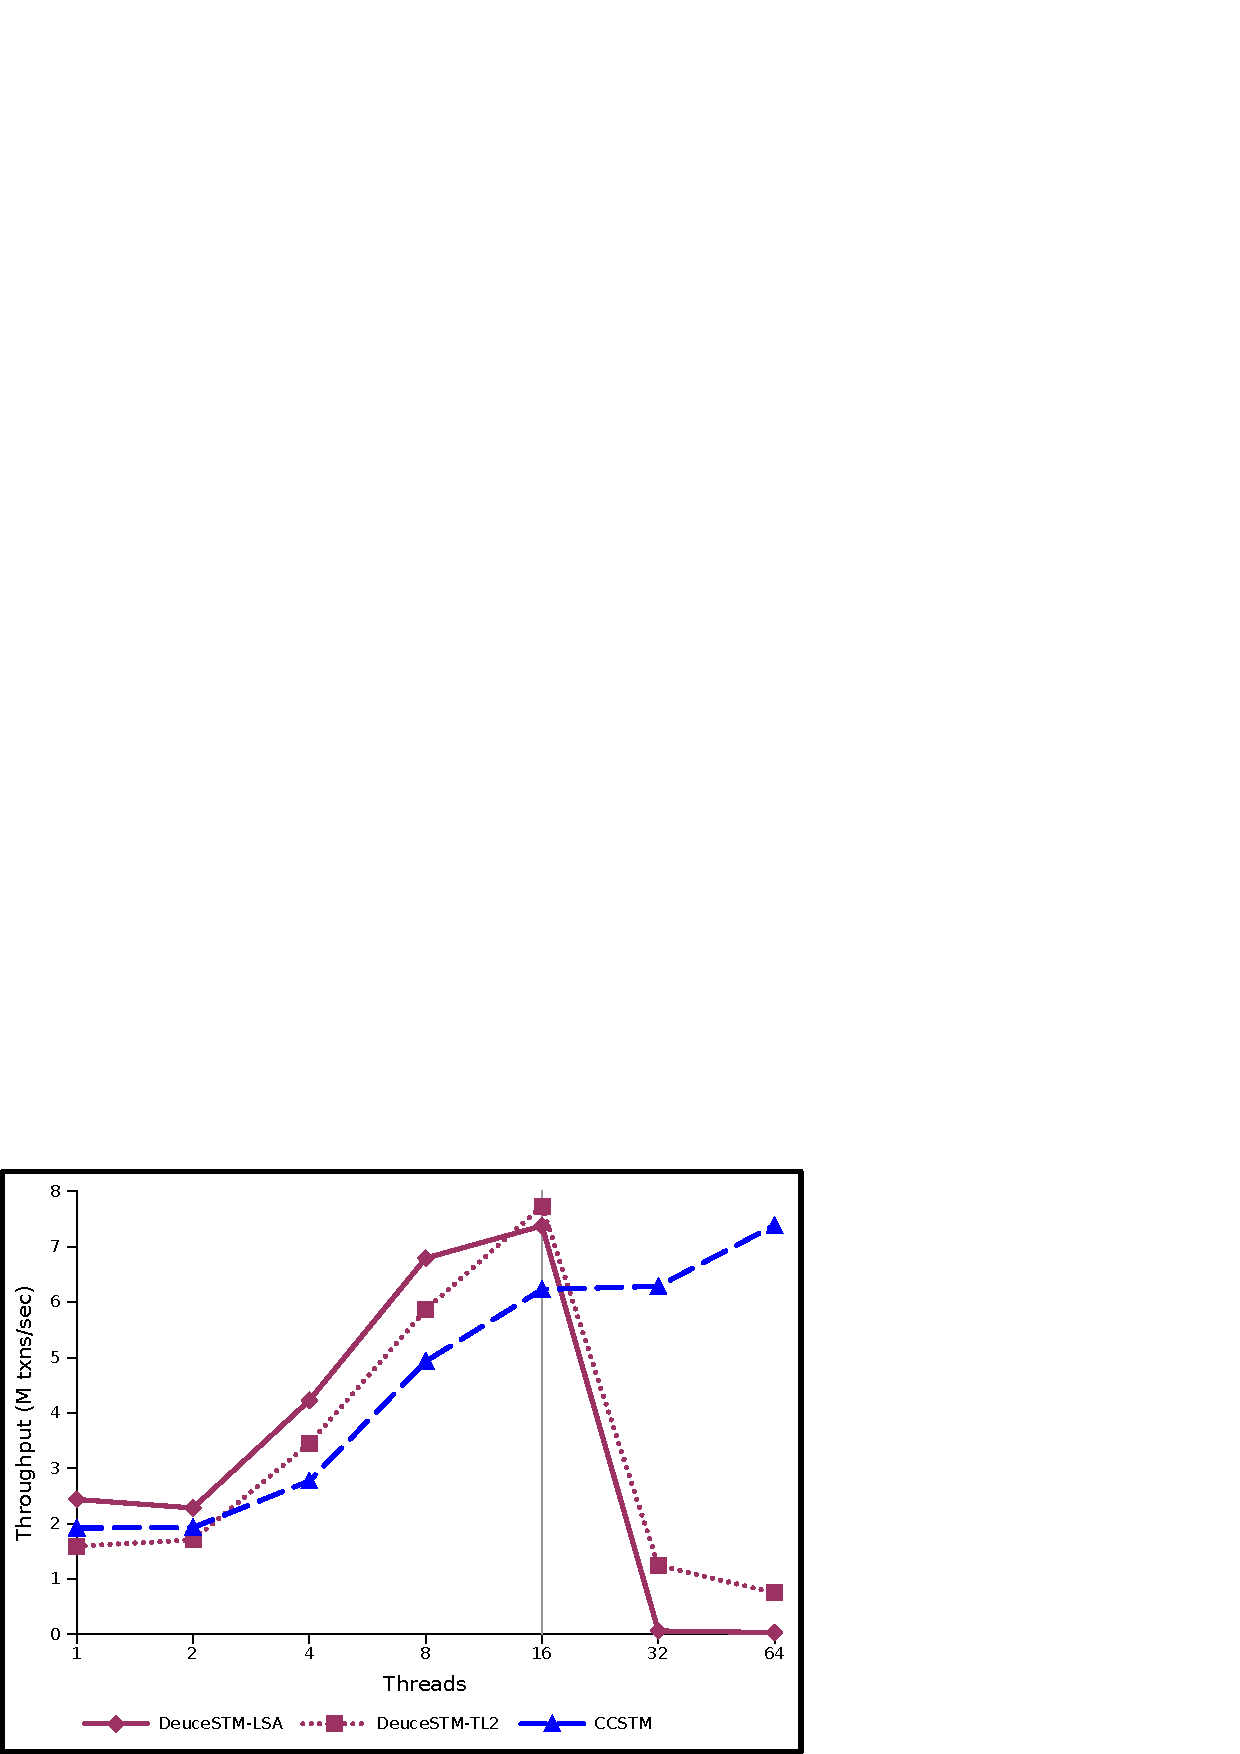
\includegraphics[clip=true,width=3in]{build/low_cont}

\caption{Throughput for the bank benchmark in a low contention scenario,
on a machine with 16 hardware thread contexts.  The number of accounts
is 64 times the number of threads.}

  \label{fig:lowcont}
\end{figure}

\begin{figure}
  \centering 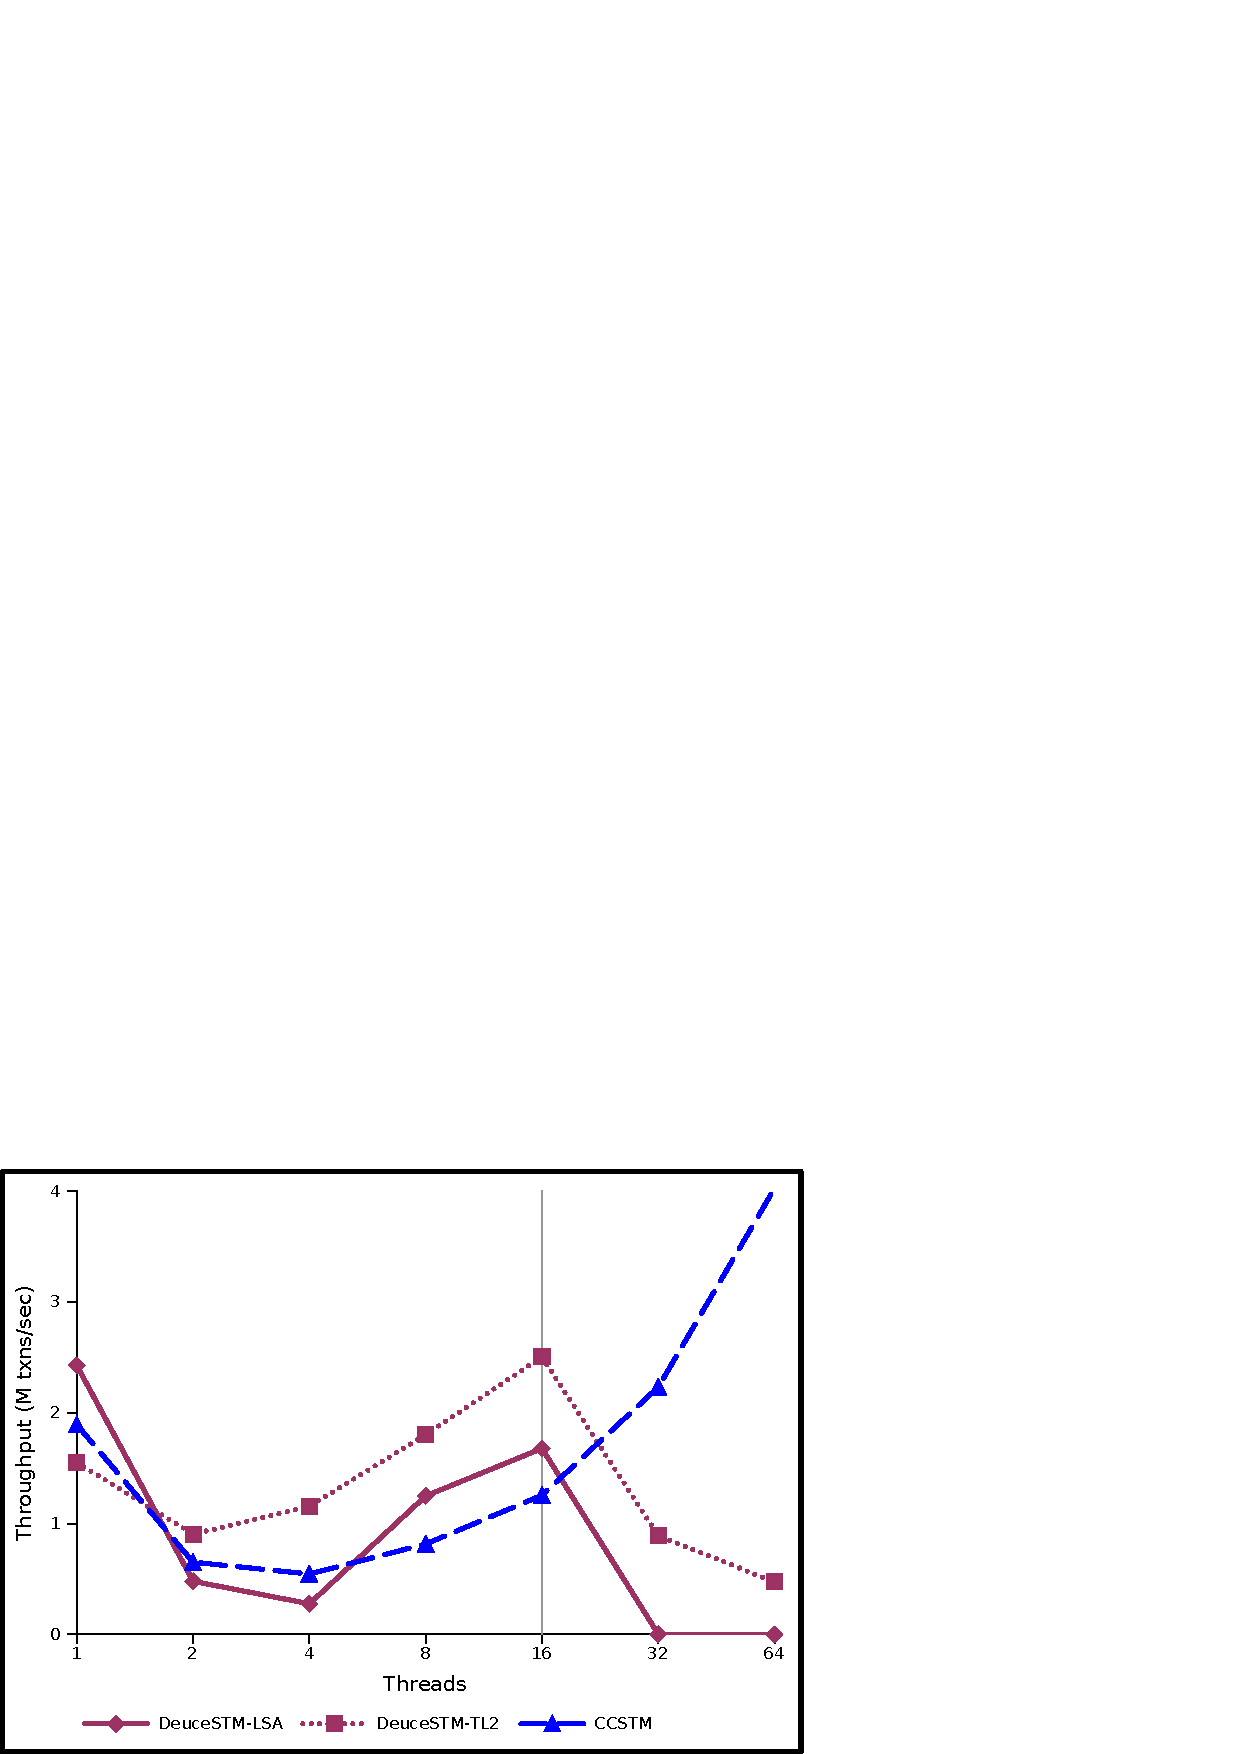
\includegraphics[clip=true,width=3in]{build/high_cont}

\caption{Throughput for a high contention scenario.  The number of accounts is
equal to the number of threads, with a minimum of two accounts.  Each
transaction touches two accounts.}

  \label{fig:highcont}
\end{figure}



\section{Discussion and Future Work}
\label{sec:discussion}

STM research is mature enough that the most difficult design decisions
for CCSTM were all found in the interface.

\subsection{Read barrier syntax}
\label{sec:syntax}

The most difficult syntactic choice was the method name for a
transactional read.  Three concise alternatives were considered:

\begin{packed_enum}

\item An implicit conversion from \xtype{Ref}{A} to \typeparam{A} -- This is
the most concise, but it interferes with further implicit conversions and type
inference for generic methods or data structures.  If \code{x} is a
\ytype{Ref}{String} holding \code{"foo"}, for example, \code{("foo" == x)}
would return false.

\item \code{unary\_!} -- A unary operator is the most concise explicit
way of denoting a read, and prefix forms of these are the only ones
that don't trigger Scala's line merging heuristic.  Initially we
settled on a \code{!} prefix for reads.  This works well for arithmetic
expressions, but it can be confusing when used in a conditional test,
as in \code{(!x == "foo")}.  It also does not chain well, requiring
extra parentheses: \code{(!x).length}.  Because of these problems, we
found ourself often reverting to the more verbose forms \code{(x.get ==
"foo")} and \code{x.get.length}.

\item \code{apply()} -- This is the only operator-like suffix method
that can safely occur at the end of the line, which means that it chains
properly in complex operations.  We initially avoided using it for read
barriers, because \code{()} is often used in Scala to help draw attention
to side-effecting methods.  Although read barriers do not themselves
perform a mutation, their access to shared mutable state also requires
extra care.  The current CCSTM code base uses \code{apply()} for concise
representation of read barriers.

\end{packed_enum}

For fields that are almost always accessed inside an atomic block, we
have also found it convenient to create transactional accessor methods.
The full \type{Ref} is published via a longer name for non-transactional
or advance operations, while the basic property name is available within
a transaction using Scala's basic field syntax:
\lstset{numbers=none}
\lstset{xleftmargin=0.125in}
\begin{lstlisting}
class Node {
  val nextRef: Ref[Node] = ..
  def next(implicit txn: Txn): Node = nextRef()
  def next_=(v: Node)(implicit txn: Txn) {
    nextRef := v 
  }
}
\end{lstlisting}
\lstset{xleftmargin=0.25in}
\lstset{numbers=left}

\color{green}
\subsection{Nested transactions}

CCSTM currently does not support nested atomic blocks, an important
omission.  A larger problem, though, is that the static scoping
of transactions would make composing such blocks difficult.  If a
method \code{m} needs a transaction internally, should it add an
\keyword{implicit} \type{Txn} parameter?  If it doesn't, then it
cannot be composed.  If it does, then the caller must always provide
an atomic block.  If the programmer wishes to provide both a simple
and a composable version of the method then he must come up with
two names.

The need for two versions of \code{m} parallels the transactional and
non-transactional access to a \type{Ref}, which was resolved there by the
\type{Ref} $\leftrightarrow$ \type{Ref.Bound} correspondence.  Rather than
coming up with two method names, the same method name can be used in
two classes.  \type{Ref}\code{.nonTxn} and \type{Ref.Bound}\code{.unbind}
convert from an instance suitable for one context to the other.  While it
may be tolerable to manage these parallel classes in the library itself,
it seems burdensome to ask the programmer to perform a similar task.

A possible solution is to provide dynamic scoping for the declaration
of atomic blocks, but static scoping for barriers.  Because nested
transactions are likely to be less common than barriers, there is less
performance motivation for avoiding the thread-local lookup.

It seems dangerous to mix static and dynamic scoping, but we notice that
for all but the most subtle uses, the static and dynamic scopes should be
identical.  This means that we can provide an execution mode that checks
the
static scopes against the dynamic ones, and triggers an exception 
if they don't match.  This checking mode would be slower on a per-barrier
basis, so like asserts it might be disabled during production use.

For applications that don't spend a large portion of their time in barriers, we
should also consider providing full dynamic scoping for transactions.
Interestingly, this could be enabled in a per-module fashion by providing an
implicit function that performs the required thread-local lookup.  The result
might look like:
\lstset{numbers=none}
\begin{lstlisting}
class Account ... {
  import STM.dynamic

  def deposit(amount: Money) {
    assert(amount >= 0)
    _balance := _balance() + amount
  }
}
\end{lstlisting}
\lstset{numbers=left}
If \code{deposit} were executed outside a transaction a runtime error would be
generated, rather than the compile-time error produced by the existing CCSTM.

Future: Partial rollback

Future: Collections

Future: Plugin

Future: @specialized

\color{black}


\section{Conclusion}
\label{sec:conclusion}

CCSTM demonstrates that it is possible to provide a library-only
implementation of STM for Scala.  The resulting
syntax is relatively concise and the performance is on par with a bytecode
rewriting STM.  The transactional references that encode CCSTM's interface
add some clutter to the user's code, but they also provide a natural way
for the programmer to take advantage of more sophisticated features such
as semantic conflict detection.

We found that the primary challenge in our approach was that statically
scoped transactions reduce composability.  The next step for CCSTM is
to explore a hybrid approach that uses static scopes for barriers but
dynamic scopes to coordinate nested transactions.



\appendix
\section{Code}

Source code for CCSTM is available under a BSD license from
\textsf{http://github.com/nbronson/ccstm} .

%%This is the text of the appendix, if you need one.

\acks

The authors would like to thank Daniel Spiewak and Peter
Veentjer for their helpful feedback during the design phase of CCSTM.

This work was supported by the Stanford Pervasive Parallelism Lab,
by Dept. of the Army, AHPCRC W911NF-07-2-0027-1, and by
the National Science Foundation under grant CNS--0720905.

{
%\small
\bibliographystyle{abbrv}
%\bibliographystyle{plainnat}
%\renewcommand{\bibfont}{\normalsize}
\bibliography{../../common/ppl}

%\begin{thebibliography}{10}
%\end{thebibliography}
}

\end{document}

